% Chapter Template

\chapter{Desarrollo: Iteración I} % Main chapter title

\label{Chapter6} % Change X to a consecutive number; for referencing this chapter elsewhere, use \ref{ChapterX}

\steveCabecera{Capítulo 6. \emph{Iteración I}} % Change X to a consecutive number; this is for the header on each page - perhaps a shortened title

%----------------------------------------------------------------------------------------
%	SECTION 1
%----------------------------------------------------------------------------------------
\section{Introducción}

En este capítulo se documentan aspectos relevantes relacionados con la codificación que se realizó en la primera iteración de desarrollo del software.\\
Se plantea la implementación reactiva y genérica de los Casos de Uso. Se expondrá sobre los Schedulers sus características y modo de empleo.
Se explicaran los Casos de Uso más interesantes de los contemplados para esta iteración.
Y se comentará sobre la implementación del repositorio de los objetos Módulo, el canal de persistencia local y el de comunicación LAN.

\section{Casos de Uso Reactivo}
Cada caso de uso escrito para la aplicación extenderá la clase abstracta \texttt{SimpleUseCase} o \texttt{CompletableUseCase} que a su vez extienden la definición genérica de un caso de uso reactivo \texttt{RxUseCase}, cuyo código depende fundamentalmente de las primitivas reactivas proporcionadas por la librería RxJava.
En la figura ~\ref{fig:class_usecases} se puede ver la relación entre las clases y la definición de los objetos de entrada y salida para cada caso de uso.

\begin{figure}[htbp]
	\centering
	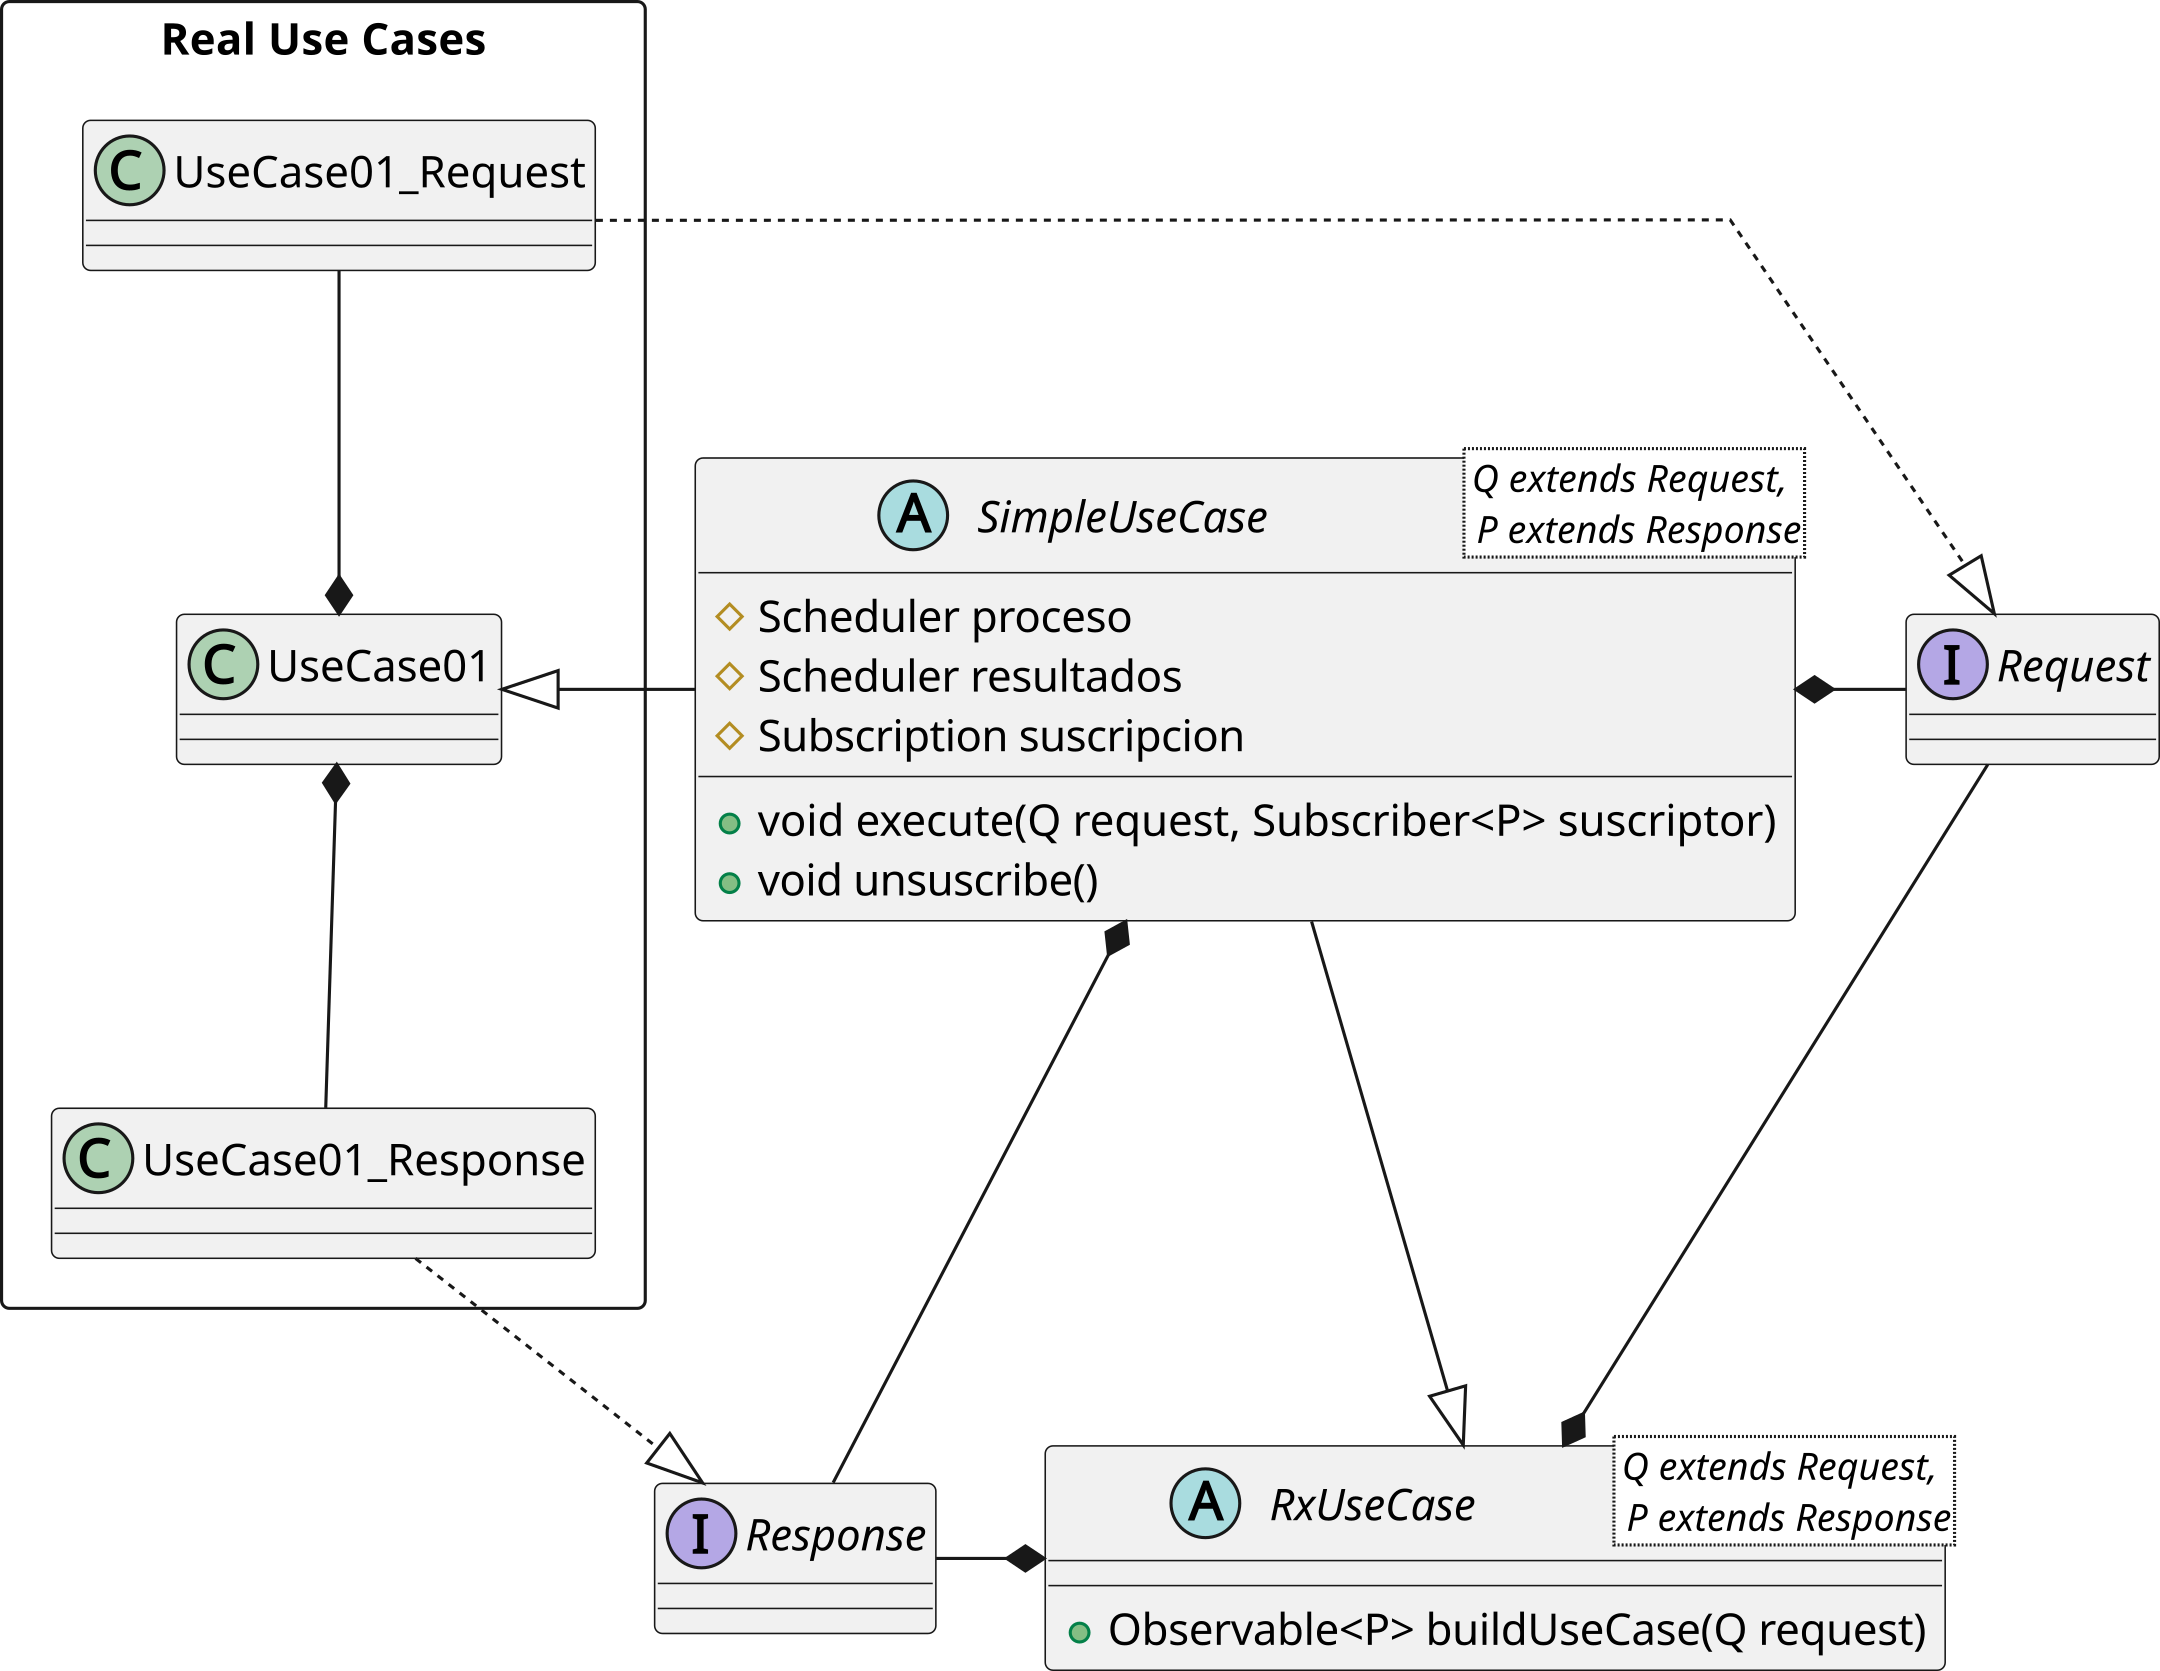
\includegraphics[width=0.8\textwidth]{Figures/iter1/CLASS_use_cases.png}
	\rule{35em}{1pt}
	\caption[Class Diagram]{Diagrama de clases de la implementación de un caso de uso.}
	\label{fig:class_usecases}
\end{figure}

\subsection{Schedulers}
En el contexto de la programación reactiva, en particular RxJava, un scheduler (planificador) es un objeto que abstrae el concepto de hilos de ejecución, controla cuándo y en qué hilo se ejecutarán las operaciones de un flujo reactivo. Es decir, proveen las instancias de hilos a las que se les asignará las tareas de los operadores en una cadena reactiva. Existen diversos Schedulers implementados por la librería, a saber:

\texttt{Schedulers.io()}\\
Optimizado para operaciones de entrada/salida (I/O), bloqueantes por definición, como llamadas de red, lectura/escritura de archivos, acceso a bases de datos, etc.
Usa un grupo de hilos que se expanden según sea necesario para acomodar la carga de trabajo I/O, y reutiliza los hilos cuando están disponibles.

\texttt{Schedulers.computation()}\\
Adecuado para operaciones computacionales que son intensivas en utilización del CPU, como cálculos matemáticos complejos.
Usa un número fijo de hilos basado en el número de núcleos del procesador, ya que tener más hilos que núcleos no mejorará el rendimiento para este tipo de tareas.

\texttt{Schedulers.newThread()}\\
Crea un nuevo hilo para cada unidad de trabajo.
No reutiliza hilos, lo que puede llevar a un consumo elevado de recursos si se usa de manera indiscriminada.

\texttt{Schedulers.single()}\\
Ejecuta todas las tareas en un solo hilo.
Útil para operaciones secuenciales donde se necesita garantizar que las tareas se ejecuten en orden sin concurrencia.

\texttt{AndroidSchedulers.mainThread()} (específico de RxAndroid)\\
Usado para ejecutar tareas en el hilo principal (UI thread) en aplicaciones Android.
Asegura que las tareas que interactúan con la UI se ejecuten en el hilo correcto.


Entendido el propósito de emplear schedulers se hace más fácil comprender la implementación del método \texttt{execute()} para la clase \texttt{SimpleUseCase}.
Cada operación de la cadena reactiva generada con \texttt{buildUseCase()} será procesada en un hilo provisto por el planificador para tareas de entrada/salida.
Así mismo las emisiones del resultado final serán capturadas por el hilo principal de la aplicación con el propósito de permitir posibles iteraciones con 
la interfaz de usuario. 

\begin{lstlisting}[caption={Método execute SimpleUseCase}, label={code:exec_usecase}, language=java, basicstyle=\ttfamily \footnotesize, numbers=left, stepnumber=1, showstringspaces=false, float]
public void execute(Q requestValues, Subscriber<P> subscriber) {
	unsubscribe();
	mSubscription = buildUseCase(requestValues)
		.subscribeOn(this.mSubscribeOn)
		.observeOn(this.mObserveOn)
		.subscribe(subscriber);
}
\end{lstlisting}

Este modo de operación multithread se especifica en las lineas 5 y 6 del código implementado para el método \texttt{excecute()} ~\ref{code:exec_usecase}
al llamar al método \texttt{subscribeOn()} se establece que todas las operaciones de la cadena reactiva se realizaran en un hilo provisto por el scheduler de E/S mientras que al llamar al método \texttt{observeOn()} como ultima operación de la cadena se fija el hilo principal de la aplicación como capturador de las emisiones del flujo de datos.

\section{Casos de Uso Implementados}
Para la presente iteración se implementaron los siguientes casos de uso.
\begin{enumerate}
	\item Buscar Módulos disponibles
	\item Solicitar Acceso
	\item Accionar Módulo
	\item Obtener datos de módulo
	\item Resetear a valores de fábrica
	\item Ingresar Credenciales WiFi
	\item Cambiar Alias	
\end{enumerate}

A continuación se documentaran aquellos que presentan los escenarios más interesantes.

\subsection{Solicitar acceso a Módulo}
Un nuevo usuario instala la aplicación cliente en su teléfono android.
Después de registrar su número telefónico, busca los módulos disponibles en la red local.
Encuentra uno y procede a solicitar acceso para que algún administrador lo autorice.
Esta operación puede utilizar hasta dos RPCs en su ejecución y puede fallar en 5 escenarios:
\begin{itemize}
	\item Error de comunicación con el módulo
	\item El módulo tuvo un error al intentar registrar al usuario
	\item Se alcanzó el máximo de usuarios admitidos por el módulo
	\item Improbable caso donde un administrador autoriza y elimina de inmediato al solicitante.
\end{itemize}
Para los escenarios 1 y 3 se permite la posibilidad de reintentar la operación una vez.
En el diagrama de la figura ~\ref{fig:act_request} se puede observar el flujo del algoritmo implementado para este caso de uso.

\begin{figure}[htbp]
	\centering
	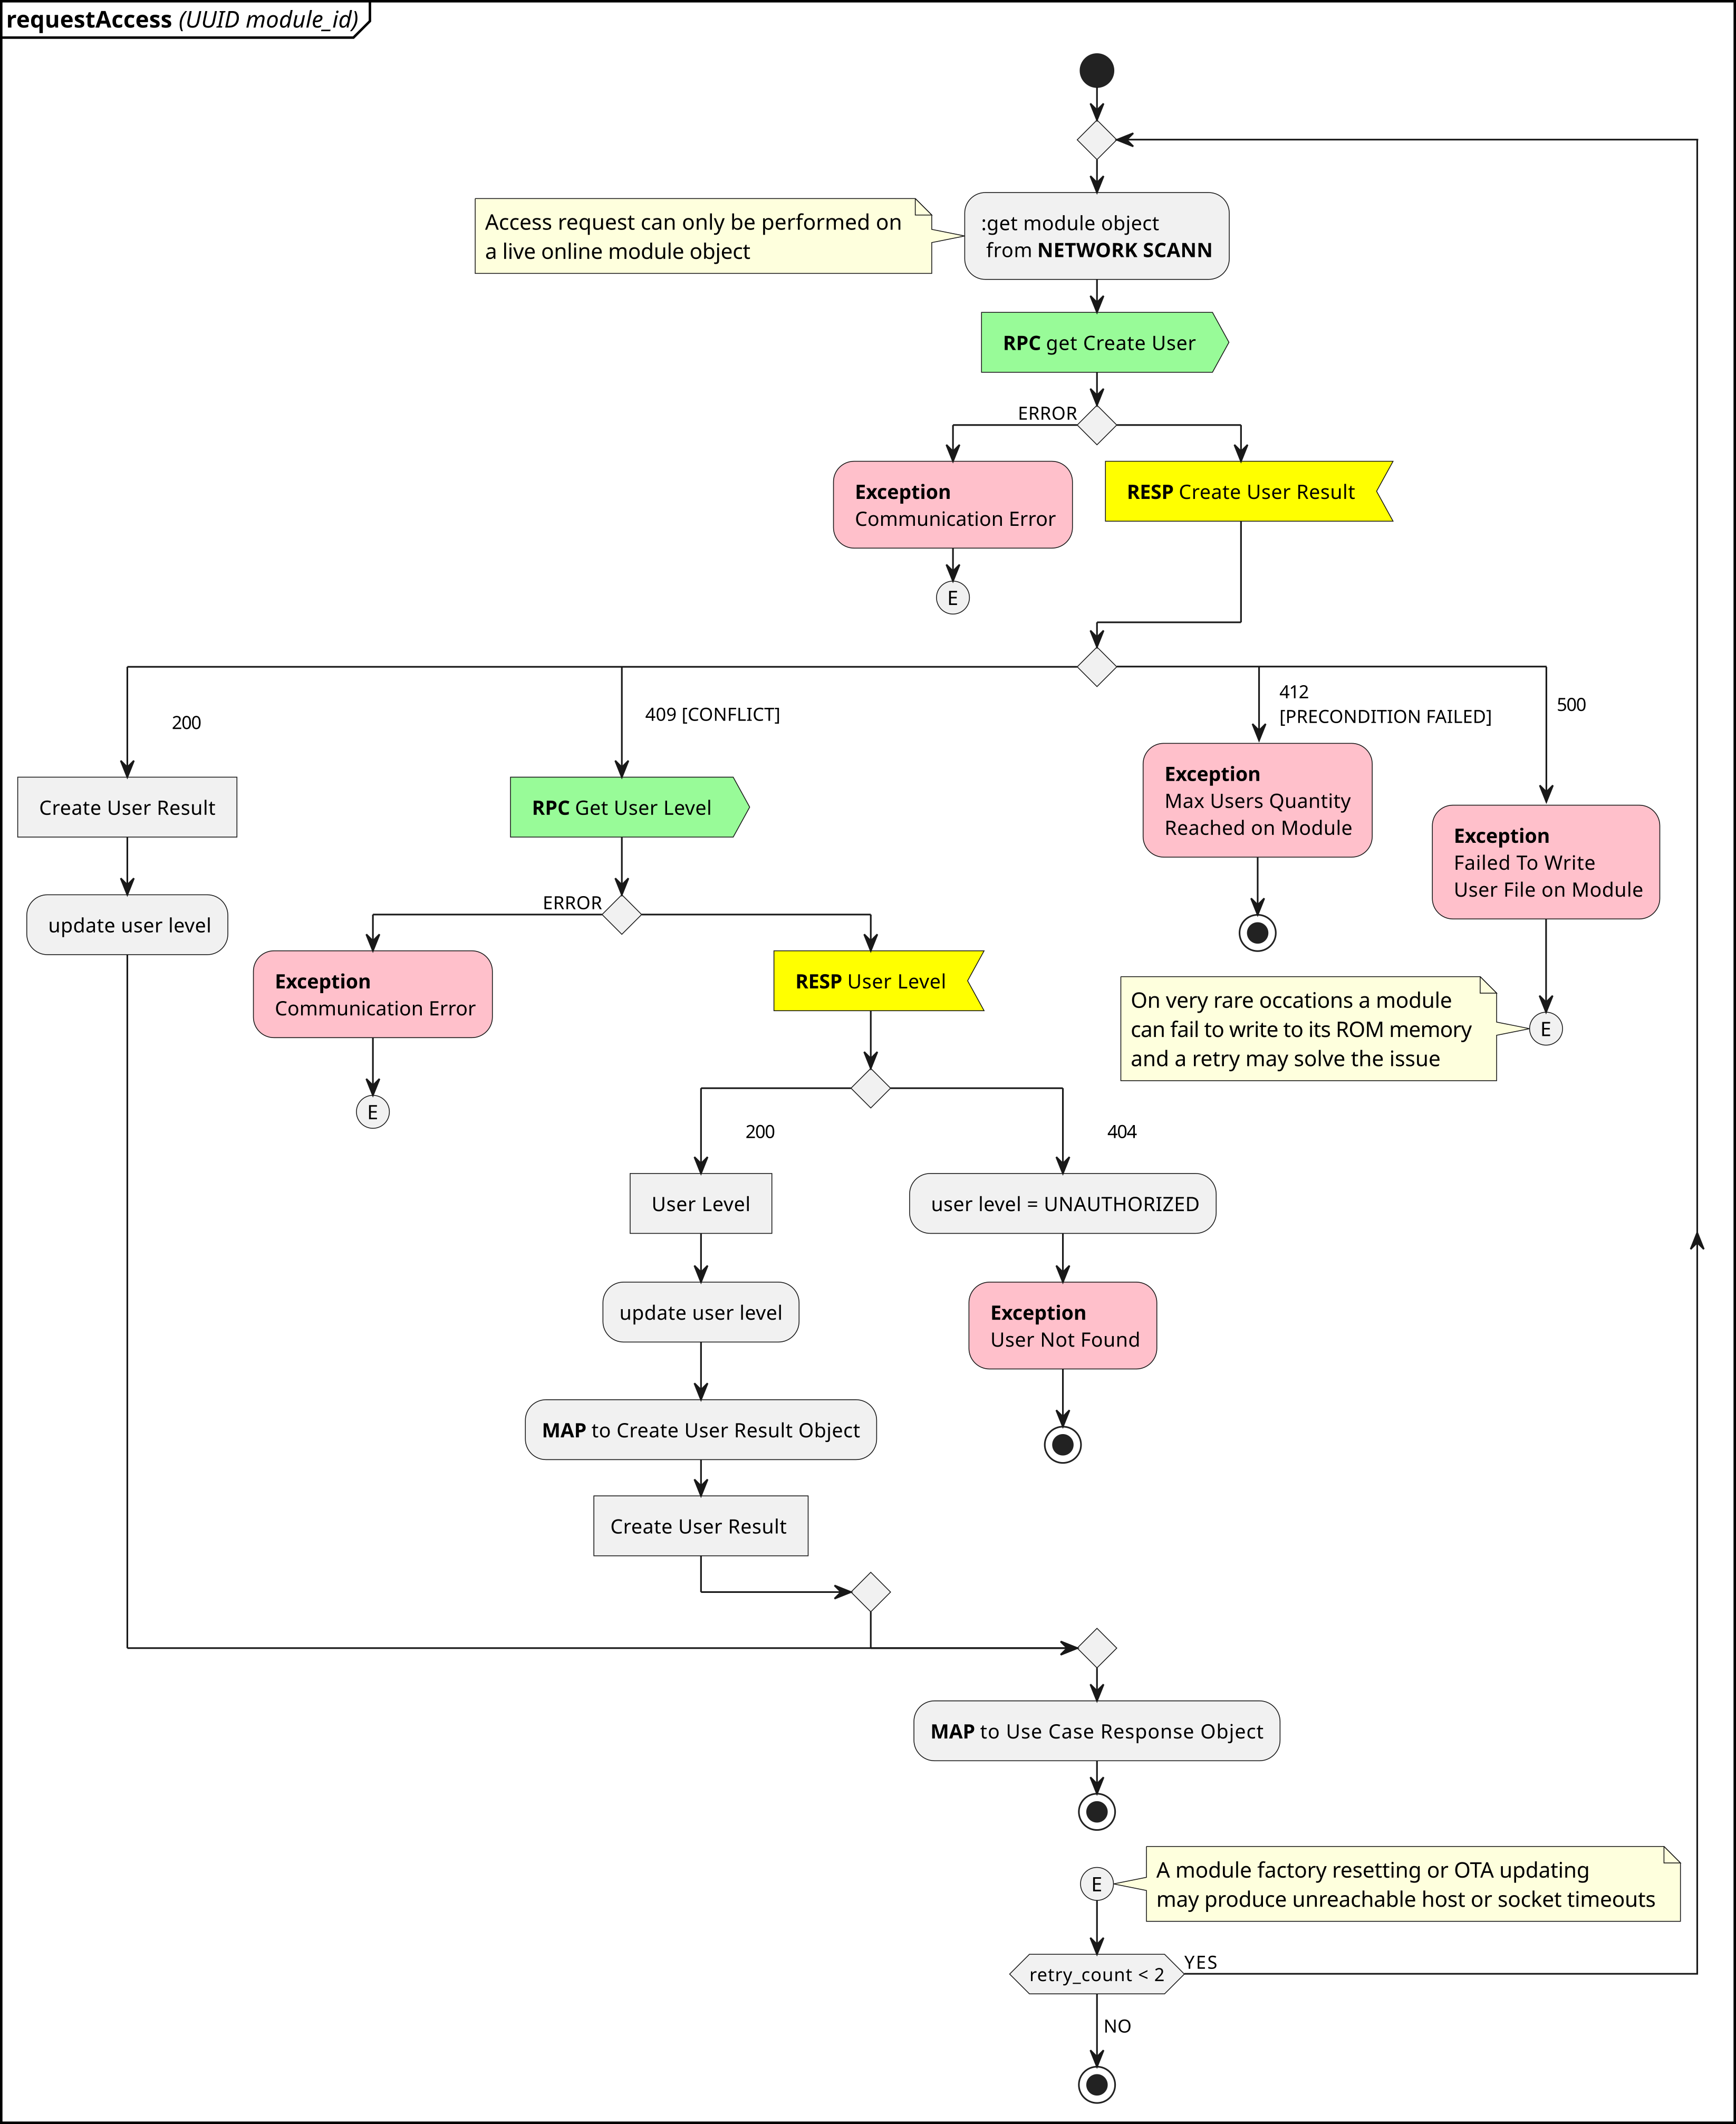
\includegraphics[width=\textwidth]{Figures/iter1/ACT_request_ink.png}
	\rule{35em}{1pt}
	\caption[Class Diagram]{Diagrama de actividades de la implementación del caso de uso: Solicitar Acceso.}
	\label{fig:act_request}
\end{figure}

\subsection{Accionar Módulo}
Un usuario abre la aplicación en su teléfono y acciona un módulo utilizando el botón deslizante.

Esta operación puede utilizar hasta dos RPCs en su ejecución y puede fallar en 3 escenarios:

\begin{enumerate}
	\item Error de comunicación con el módulo.
	\item El usuario que intenta accionar el módulo no existe.
	\item El usuario ha cambiado de nivel.
\end{enumerate}

Para los escenarios 1 y 3 se admite la posibilidad de reintentar la operación una vez.
En el diagrama de la figura ~\ref{fig:act_trigger} se puede observar el flujo del algoritmo implementado para este caso de uso.

\begin{figure}[htbp]
	\centering
	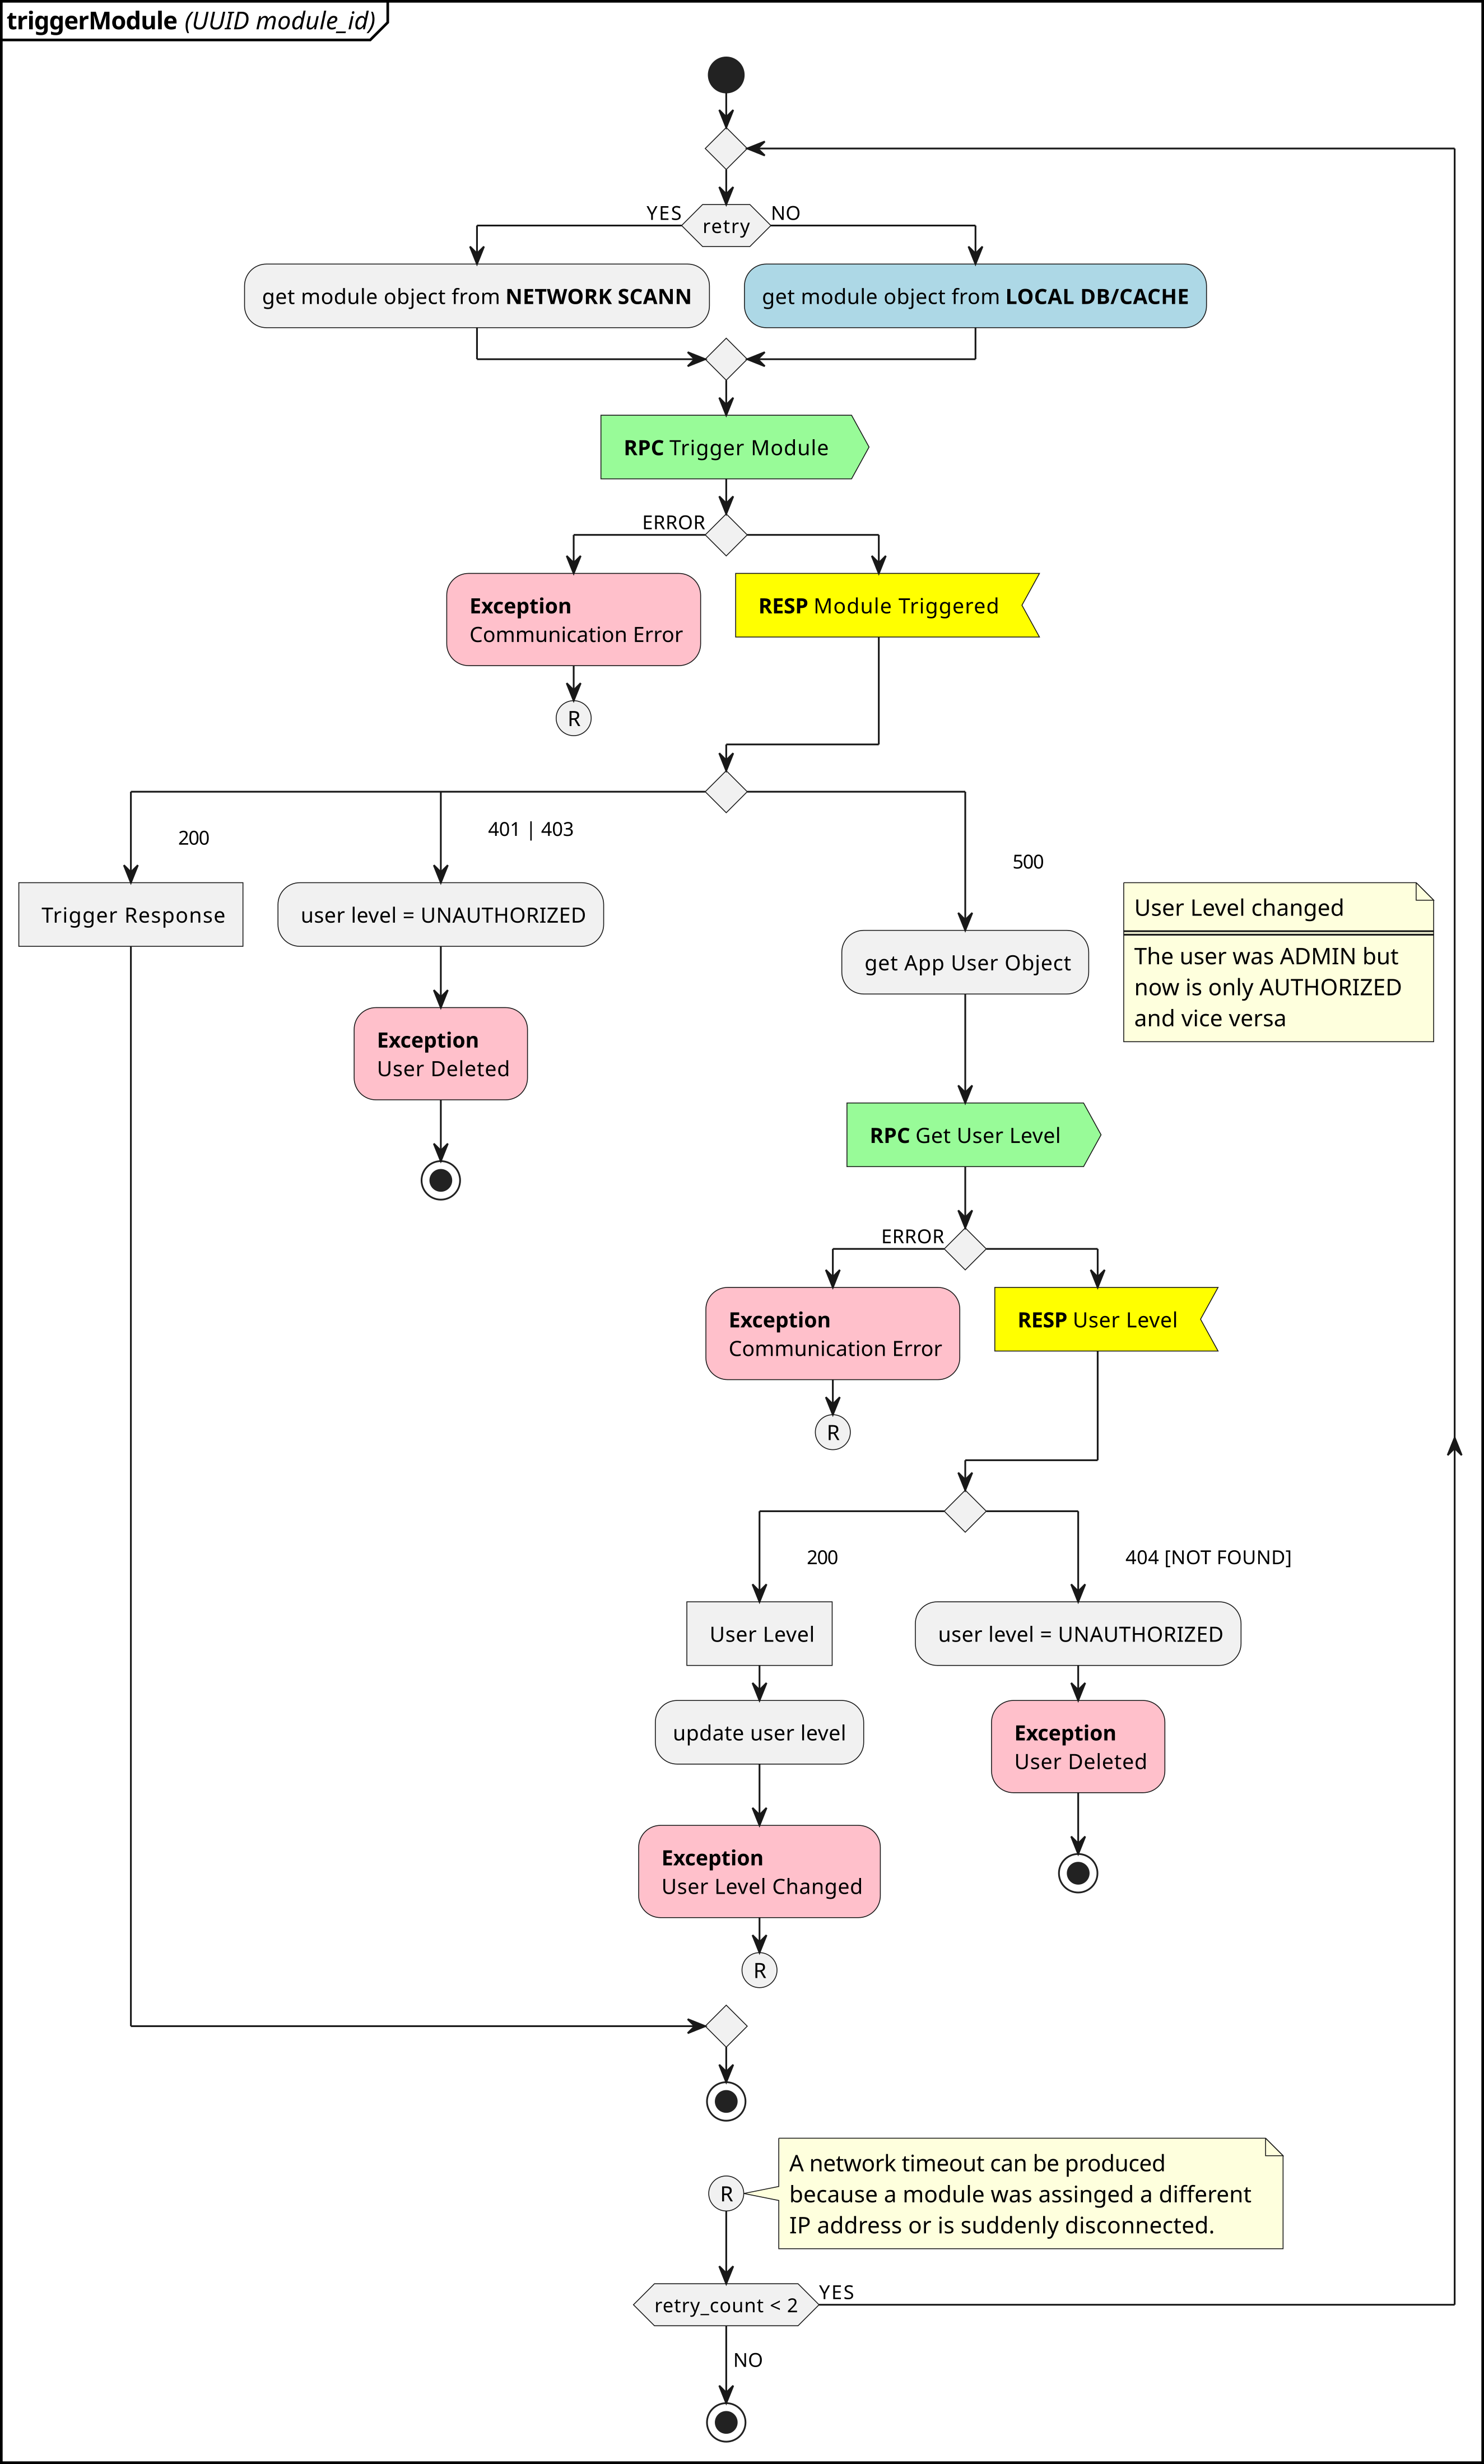
\includegraphics[width=0.8\textwidth]{Figures/iter1/ACT_trigger_module.png}
	\rule{35em}{1pt}
	\caption[Class Diagram]{Diagrama de actividades de la implementación del caso de uso: Accionar Módulo.}
	\label{fig:act_trigger}
\end{figure}

\subsection{Obtener datos del Módulo}
Un usuario toca el botón con forma de engranaje circular para acceder a las configuraciones de un módulo en particular.
Se distinguen los dos escenarios correspondientes a los modos de funcionamiento: la configuración inicial y la operación regular, descritos en la sección ~\ref{section:interfaces}.
Con el objetivo de obtener los parámetros actualizados del módulo se realizan varias operaciones en background para asegurar la consistencia de los datos y construir la UI adecuada para tal caso.

Esta operativa puede utilizar hasta tres RPCs en su ejecución y puede fallar en seis escenarios con cuatro tipos de error:

\begin{enumerate}
	\item Aplicación no conectada a módulo en configuración inicial.
	\item Error de comunicación con el módulo.
	\item El Usuario que realiza la consulta fue eliminado.
	\item Formato de consulta RPC erróneo.
\end{enumerate}

En el diagrama de la figura ~\ref{fig:act_get_umod_data} se puede observar el flujo del algoritmo implementado para este caso de uso.

\begin{figure}[htbp]
	\centering
	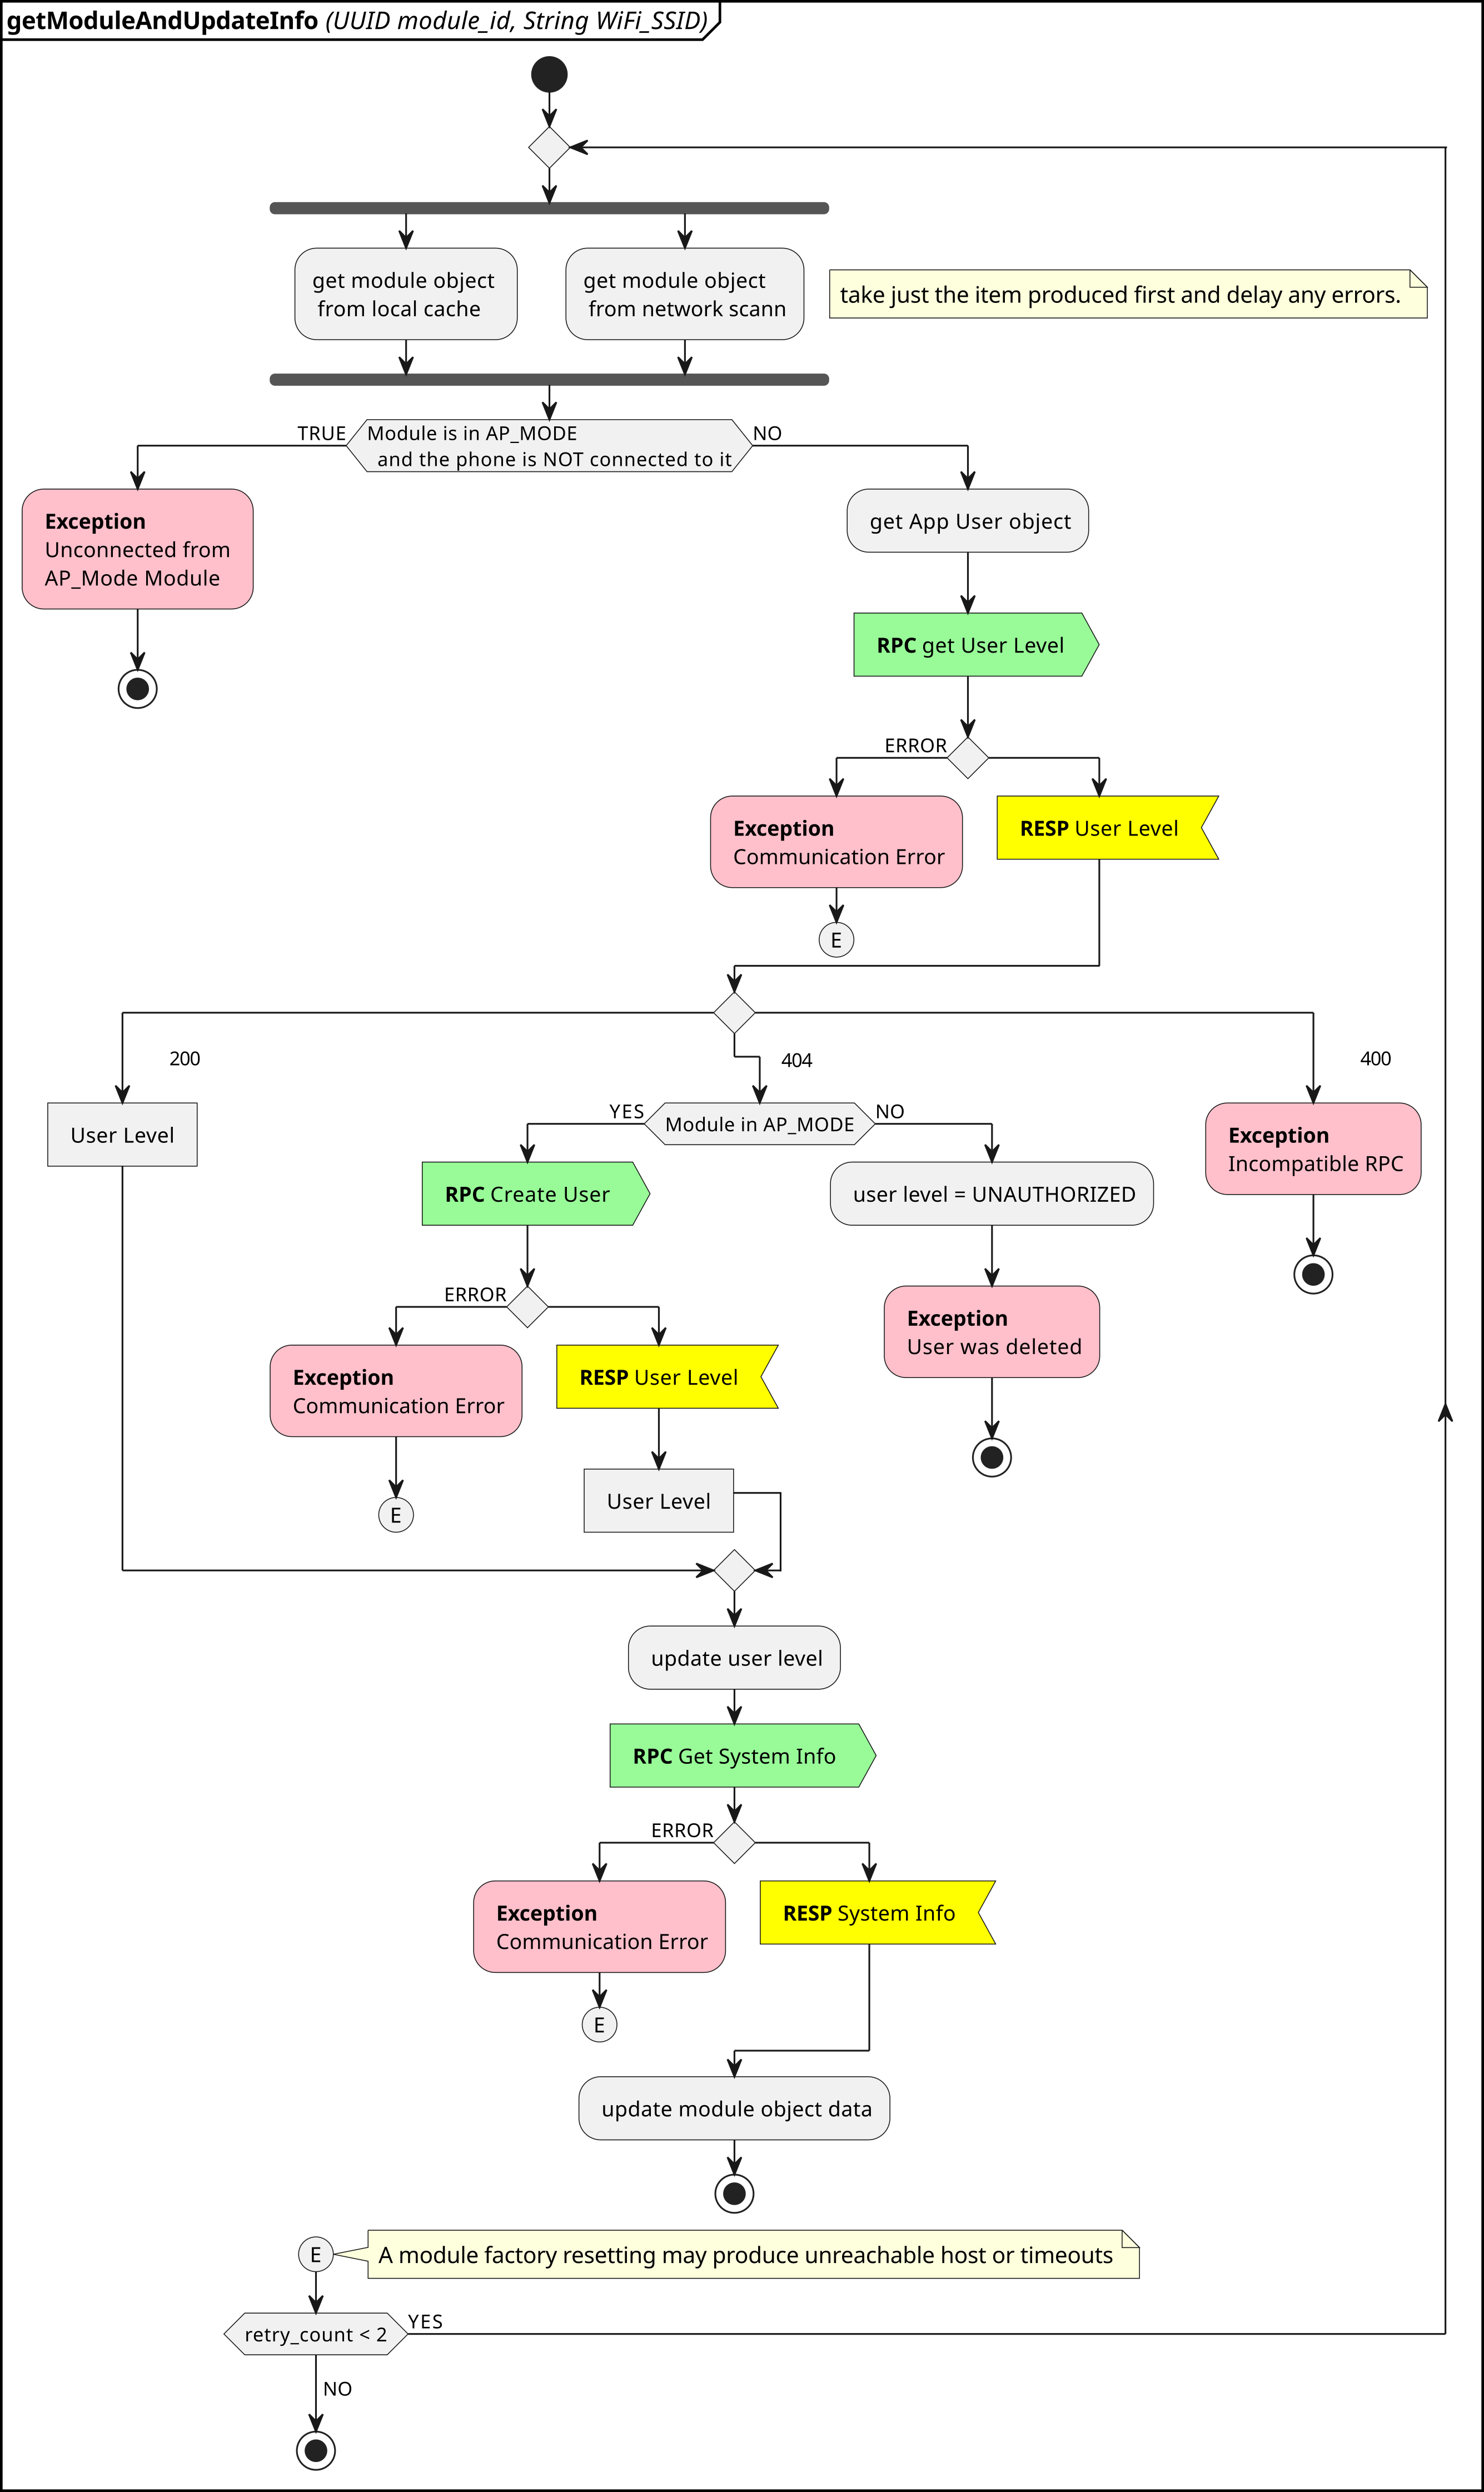
\includegraphics[width=0.8\textwidth]{Figures/iter1/ACT_getModuleAndUpdateInfo_ink.png}
	\rule{35em}{1pt}
	\caption[Class Diagram]{Diagrama de actividades de la implementación del caso de uso: Accionar Módulo.}
	\label{fig:act_get_umod_data}
\end{figure}

\section{Repositorio Objetos Módulo}
\subsection{Objeto Módulo: UMod}
Los módulos electrónicos se representan en el código de la aplicación como objetos de tipo UMod 
estas entidades mantendrán registro de tres atributos enumerados a saber.
\begin{enumerate}
	\item \textbf{STATE}: es un reflejo exacto de la máquina de estados implementada en el firmware del módulo.
	\item \textbf{STATUS}: hace referencia al reporte de apertura del sistema dónde está instalado el módulo.
	\item \textbf{SOURCE}: indica el origen de la última actualización de este objeto.
\end{enumerate}

\begin{figure}[htbp]
	\centering
	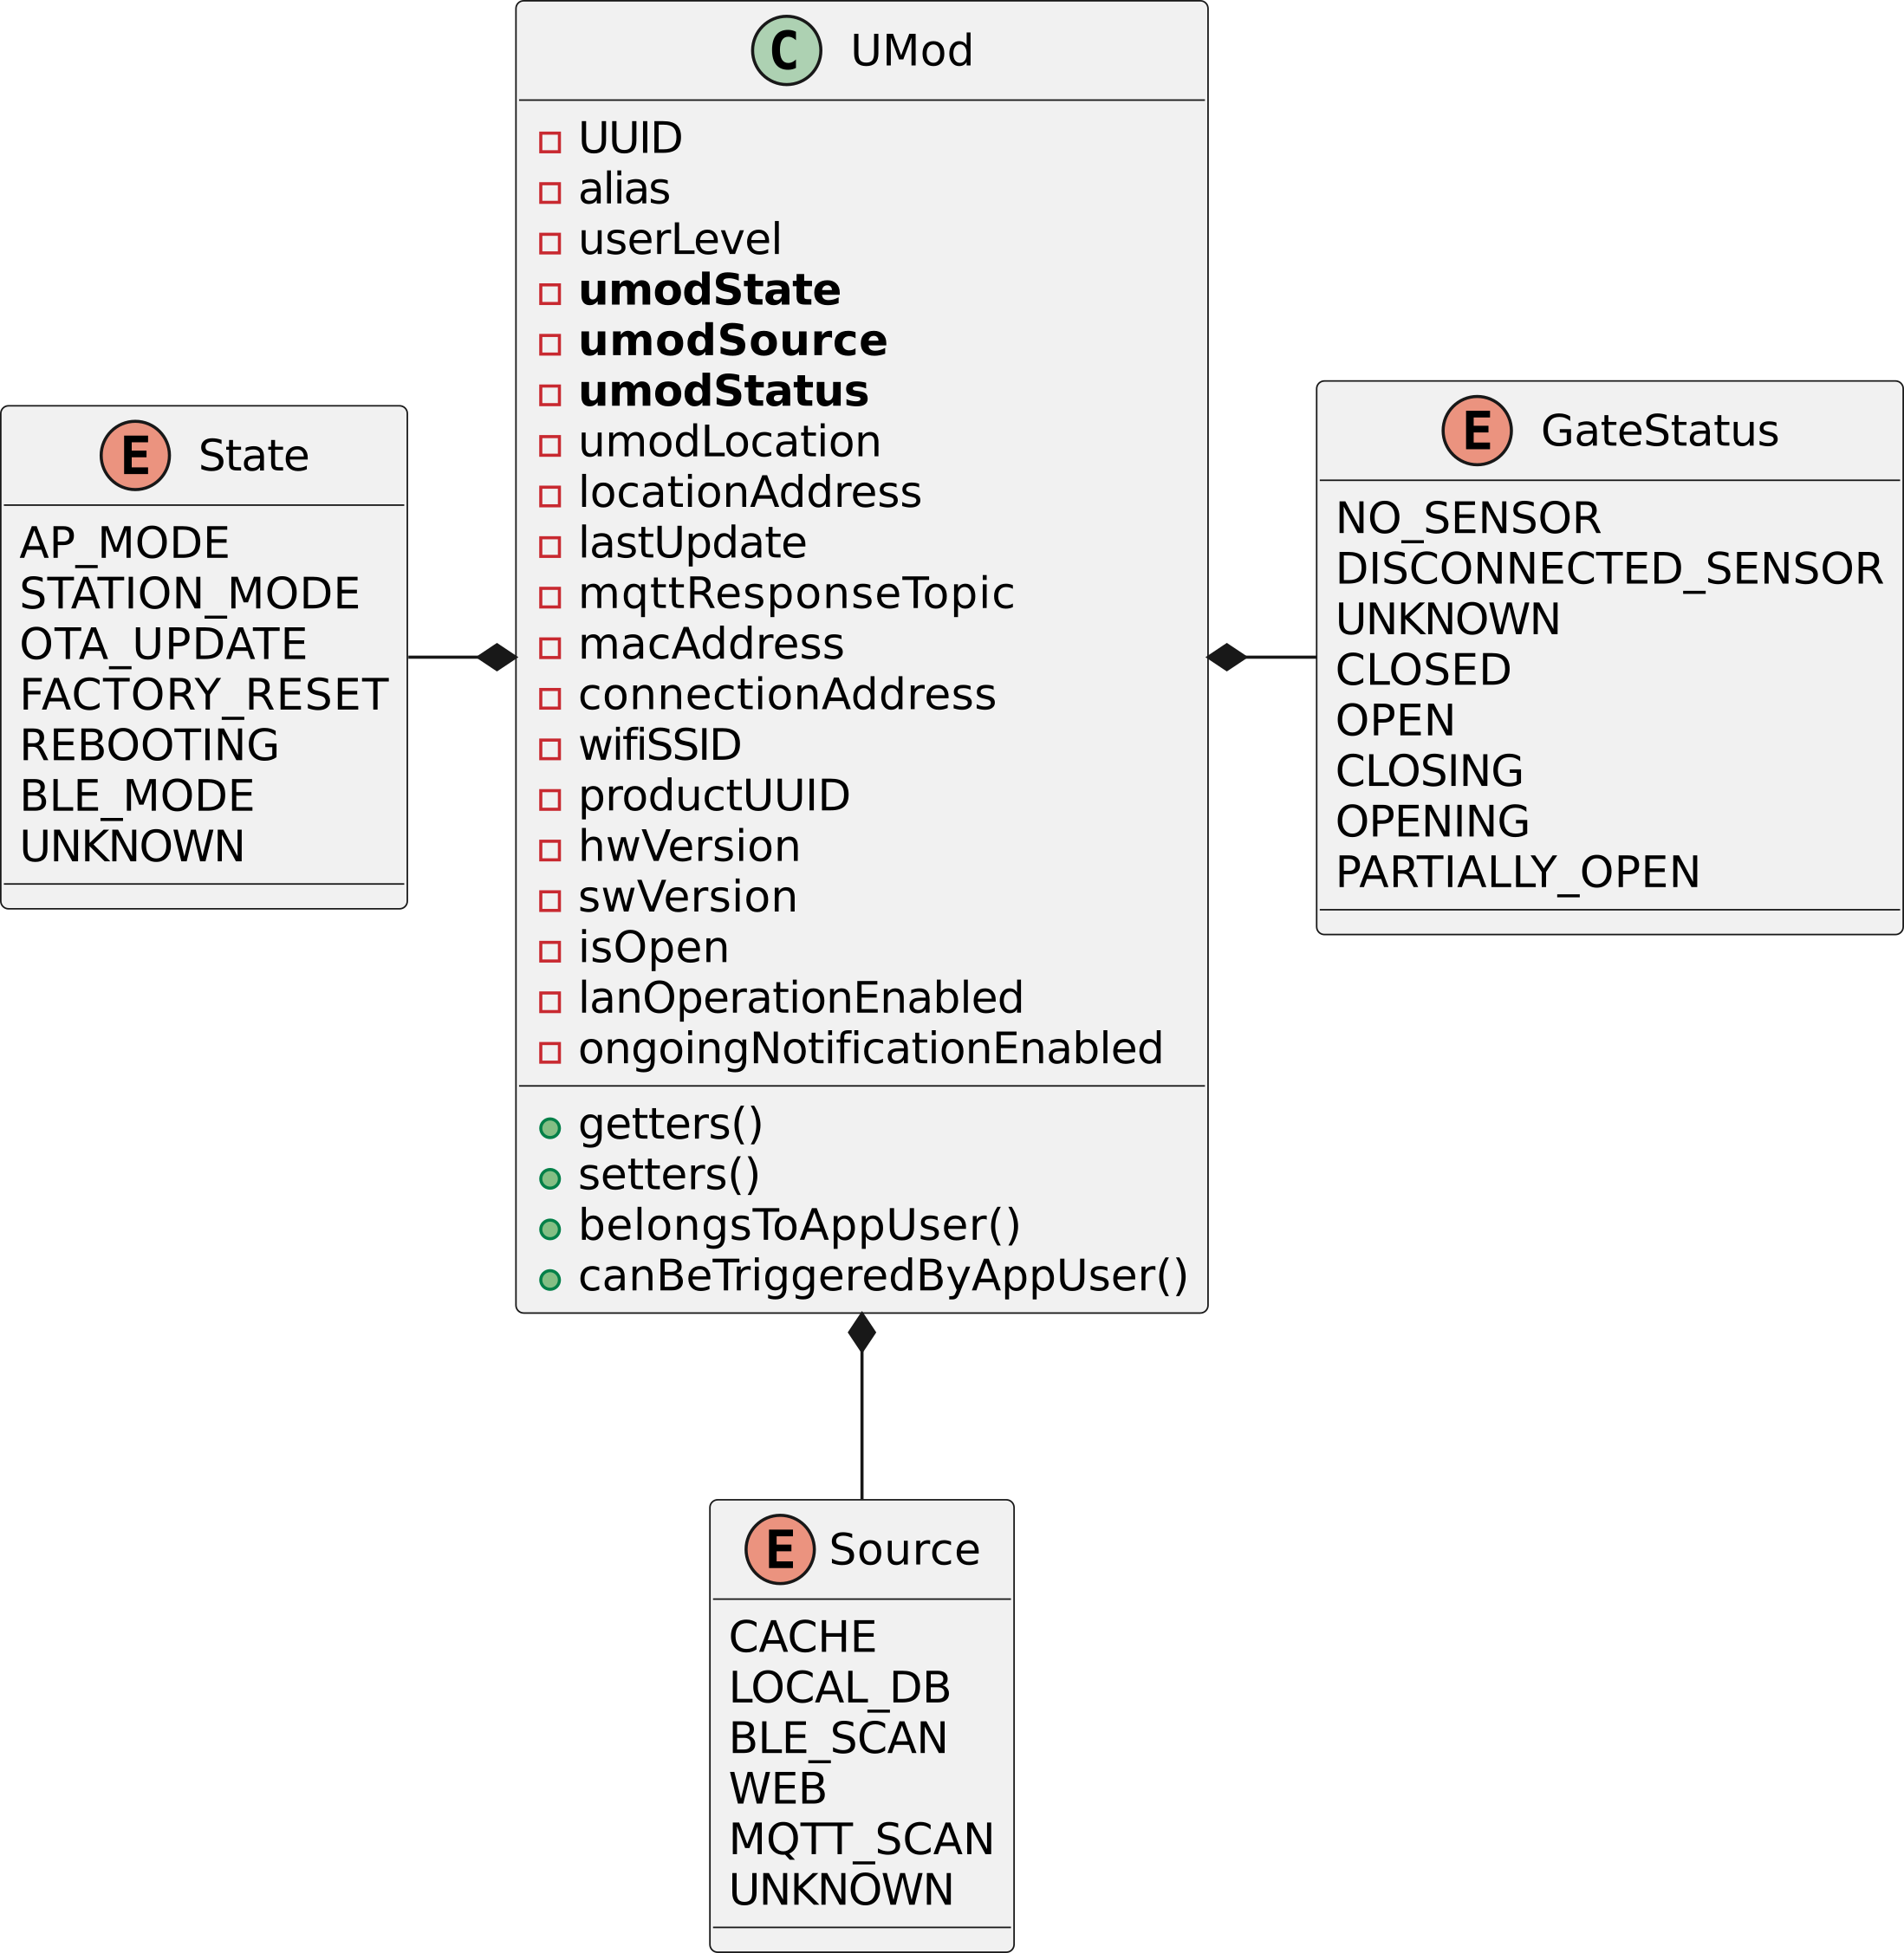
\includegraphics[width=0.7\textwidth]{Figures/iter1/CLASS_umod_ink.png}
	\rule{35em}{1pt}
	\caption[Class Diagram]{Diagrama de clases de la implementación del Objeto Módulo.}
	\label{fig:class_umod}
\end{figure}

Los demás atributos se muestran el la figura ~\ref{fig:class_umod} son auto-descriptivos y serán utilizados para popular la interfaz gráfica y para realizar las operaciones soportadas por la aplicación.

\subsection{Repositorio}
Las operaciones CRUD de estos objetos son responsabilidad del objeto repositorio que debería instanciarse a modo \texttt{singleton} para asegurar la consistencia de sus operaciones. Tal como fue introducido en la sección de diseño ~\ref{section:repository}, las tareas de persistencia y comunicación con los objetos módulo se implementarán utilizando el patrón de diseño \texttt{repository} con las modificaciones documentadas. Si se comparan las figuras ~\ref{fig:uml_clases_modif_repository} y ~\ref{fig:class_umods_repository} puede observarse como la implementación en el código de la aplicación respeta tal diseño. Se escribirán cada una de las operaciones soportadas como RPC en métodos individuales, en el diagrama de clases solo se muestra uno a modo ilustrativo.

\begin{figure}[htbp]
	\centering
	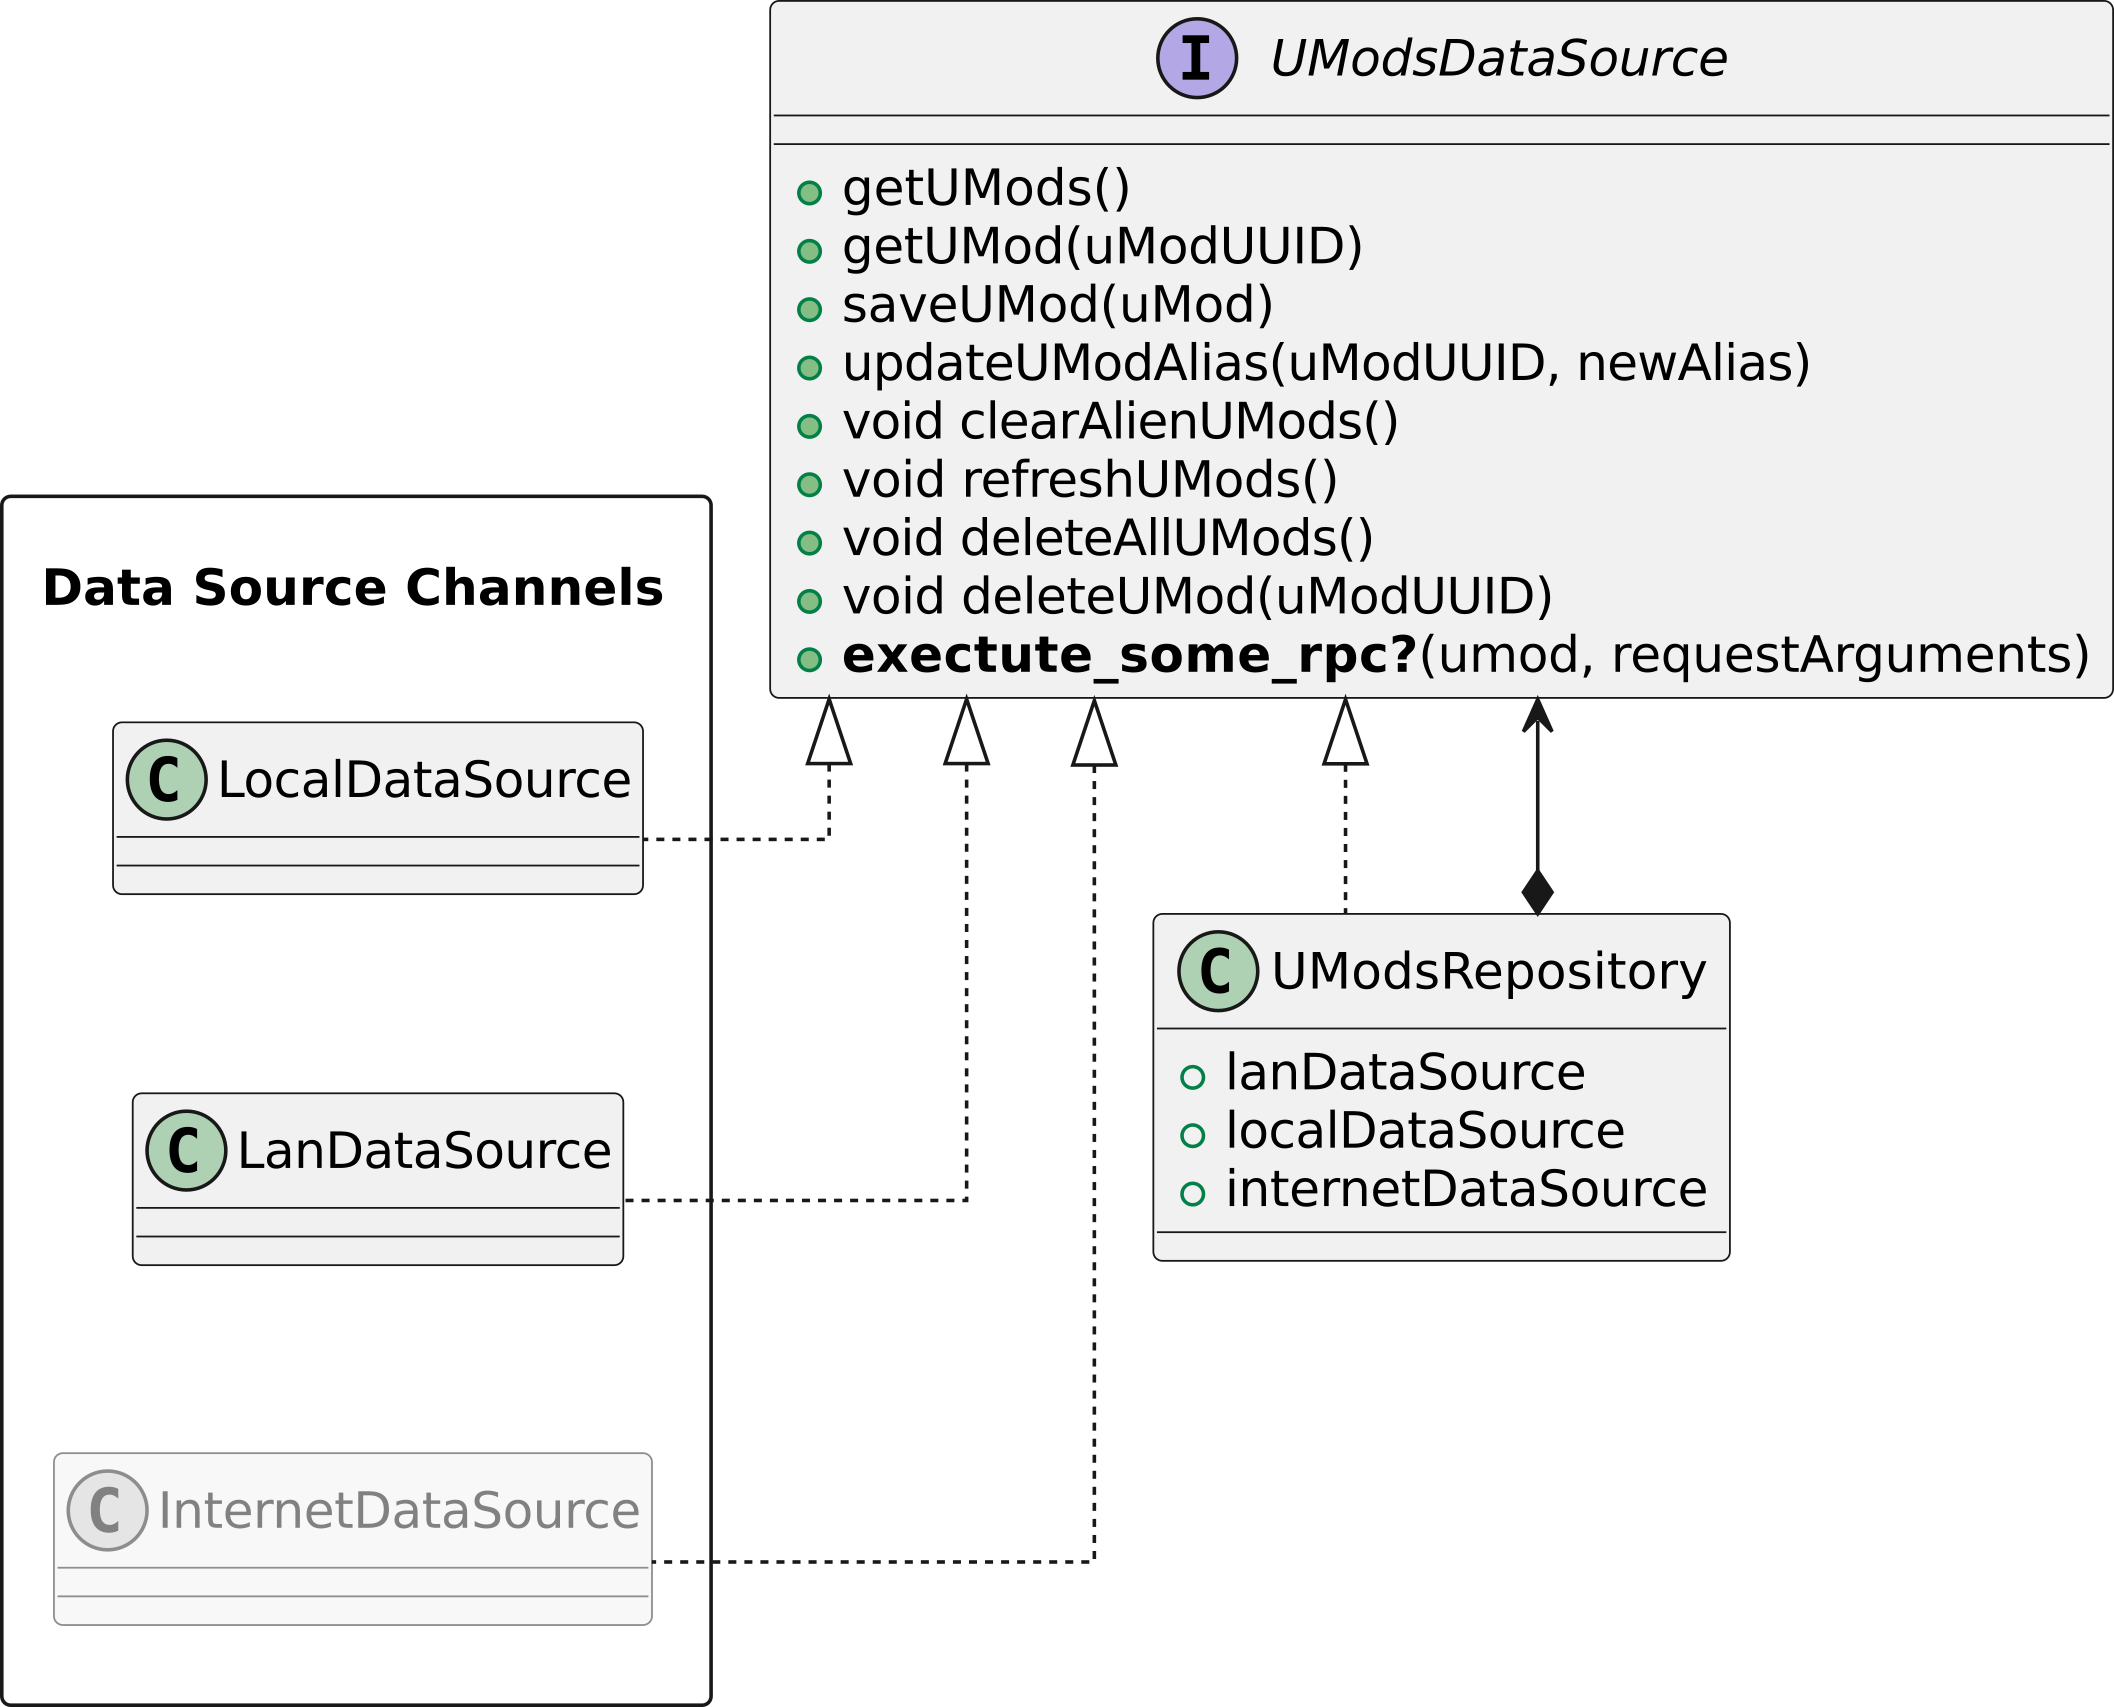
\includegraphics[width=0.7\textwidth]{Figures/iter1/CLASS_umods_repository_ink.png}
	\rule{35em}{1pt}
	\caption[Class Diagram]{Diagrama de clases de la implementación del Repositorio para los objetos módulo.}
	\label{fig:class_umods_repository}
\end{figure}

Dado que todos los canales de origen de datos para el repositorio fueron implementados como emisores reactivos se hace un uso intensivo de operadores sobre flujos reactivos. Se evidencian tanto la complejidad como la gran utilidad de el empleo de este paradigma.

\subsubsection{Canal de Persistencia Local}
Para mantener un registro local de módulos configurados y utilizados por el usuario es necesario utilizar alguna forma de persistencia local en el dispositivo. Se optó por utilizar sqlite y un wrapper reactivo para acceder a la base de datos. Los módulos configurados son almacenados en las filas de una única tabla. Como todos los canales de datos implementan la misma interfaz \texttt{UModuleDataSource} los métodos asignados a la ejecución de los RPC quedan vacíos para este canal. 

\subsubsection{Canal de Comunicación de Área Local}
Con el objetivo de poder ejecutar los protocolos remotos (RPCs) se declara un canal para comunicación HTTP.
Para ello se utilizó la librería Retrofit que provee un wrapper reactivo out-of-the-box y permite la configuración de las
solicitudes http a modo declarativo dejando oculto los pormenores del protocolo de comunicación.
Fue necesario incorporar un interceptor de solicitudes para habilitar el método de autenticación por digesto documentado en la sección ~\ref{section:digest}.